% Generated by course-project/tools/report_assets.py from the evidence files; do not edit by hand.

\begin{figure}[t]
\centering
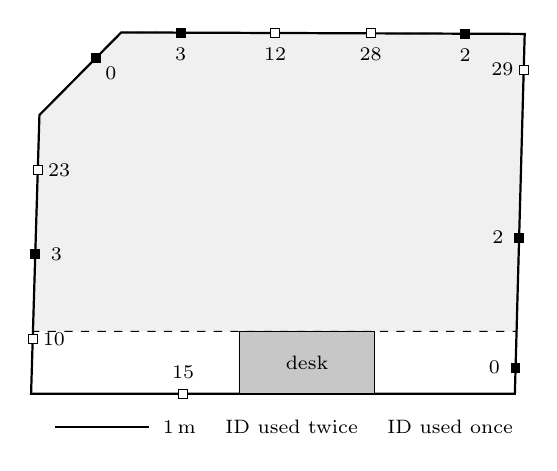
\begin{tikzpicture}[font=\scriptsize, x=1cm, y=1cm]
\fill[black!6] (0.024,0.792) -- (0.106,3.540) -- (1.145,4.589) -- (6.269,4.570) -- (6.166,0.792) -- cycle;
\draw[dashed, line width=0.4pt] (0.024,0.792) -- (0.106,3.540) -- (1.145,4.589) -- (6.269,4.570) -- (6.166,0.792) -- cycle;
\draw[line width=0.8pt] (0.000,0.000) -- (0.106,3.540) -- (1.145,4.589) -- (6.269,4.570) -- (6.144,0.000) -- cycle;
\draw[fill=black!22, line width=0.4pt] (2.652,0.000) rectangle (4.356,0.792);
\node at (3.504,0.396) {desk};
\node[draw, fill=white, minimum size=3.2pt, inner sep=0pt] at (1.932,0.000) {};
\node[inner sep=0pt] at (1.932,0.270) {15};
\node[draw, fill=white, minimum size=3.2pt, inner sep=0pt] at (0.020,0.696) {};
\node[inner sep=0pt] at (0.290,0.688) {10};
\node[draw, fill=black, minimum size=3.2pt, inner sep=0pt] at (0.053,1.775) {};
\node[inner sep=0pt] at (0.323,1.767) {3};
\node[draw, fill=white, minimum size=3.2pt, inner sep=0pt] at (0.085,2.843) {};
\node[inner sep=0pt] at (0.355,2.835) {23};
\node[draw, fill=black, minimum size=3.2pt, inner sep=0pt] at (0.823,4.265) {};
\node[inner sep=0pt] at (1.015,4.075) {0};
\node[draw, fill=black, minimum size=3.2pt, inner sep=0pt] at (1.901,4.586) {};
\node[inner sep=0pt] at (1.900,4.316) {3};
\node[draw, fill=white, minimum size=3.2pt, inner sep=0pt] at (3.101,4.582) {};
\node[inner sep=0pt] at (3.100,4.312) {12};
\node[draw, fill=white, minimum size=3.2pt, inner sep=0pt] at (4.313,4.577) {};
\node[inner sep=0pt] at (4.312,4.307) {28};
\node[draw, fill=black, minimum size=3.2pt, inner sep=0pt] at (5.513,4.572) {};
\node[inner sep=0pt] at (5.512,4.302) {2};
\node[draw, fill=black, minimum size=3.2pt, inner sep=0pt] at (6.152,0.324) {};
\node[inner sep=0pt] at (5.883,0.332) {0};
\node[draw, fill=black, minimum size=3.2pt, inner sep=0pt] at (6.198,1.979) {};
\node[inner sep=0pt] at (5.928,1.986) {2};
\node[draw, fill=white, minimum size=3.2pt, inner sep=0pt] at (6.257,4.115) {};
\node[inner sep=0pt] at (5.987,4.122) {29};
\draw[line width=0.6pt] (0.300,-0.42) -- (1.500,-0.42);
\node[anchor=west] at (1.550,-0.42) {1\,m};
\node[anchor=west] at (2.250,-0.42) {$\blacksquare$ ID used twice\quad $\square$ ID used once};
\end{tikzpicture}
\caption{The real arena seen from above, with the 12 nominal AprilTag positions and their IDs. The dashed outline is the driving area. The tags are printed but not yet mounted; the world file will use the centers measured after mounting.}
\label{fig:room}
\end{figure}
